\documentclass[11pt]{article}
\usepackage{graphicx}
\usepackage{natbib}
\usepackage{lscape}
\renewcommand{\topfraction}{0.85}
\renewcommand{\textfraction}{0.1}
\oddsidemargin=0.5cm \topmargin=0cm \setlength{\textheight}{21cm}
\setlength{\textwidth}{15.5cm}
\renewcommand{\baselinestretch}{1.2}
\renewcommand{\figurename}{Exhibit}
\renewcommand{\tablename}{Exhibit}
\usepackage{amsmath}

\begin{document}

{\bf  \large \noindent EXHIBITS}

\setcounter{page}{17}


\bigskip


\begin{figure}[h]
\begin{center}
\caption{Percentage CVaR contribution of asset 1 in function of its portfolio weight for a two-asset portfolio with asset returns that have a bivariate normal distribution with means $\mu_1$ and $\mu_2$, correlation $0.5$ and standard deviations $\sigma_1$ and $\sigma_2$, respectively.   }
\includegraphics[width=9cm,angle=270]{sensitivity_rho50.eps}
\end{center}
\end{figure}


\newpage

\begin{figure}[tb]
\begin{center}
\caption{Weight and CVaR allocation of bond-equity portfolios, together with the in-sample annualized monthly mean and monthly 95\% CVaR over
the period January 1976-June 2010.     }
\vspace{1cm}
\scalebox{0.87}{
\begin{tabular}{|lc cc c cc c cc | } \hline
                          &  &	\multicolumn{2}{c}{Weight allocation} 	& &\multicolumn{2}{c}{CVaR allocation} & & Ann. mean & 95\% CVaR  \\
                         &  &	Bond & Equity 	& &Bond & Equity 	& &  & \\ \hline
Equal-weight	        &    &50\%  	&50\%       &	&3.47\%  & 96.53\% & & 8.90\% & 4.87\% \\
60/40 weight            &    &40\%  	&60\%       &  & 0\%     & 100\%   & & 9.17\% & 5.82\%\\
Min CVaR                &	 &96.86\%	& 3.14\%    &  & 96.86\%    & 3.14\%  & & 7.63\% & 2.44\%\\
Min CVaR concentration	&    &77.01\%	&22.91\%    &  & 50\%	     &50\%     & & 8.17\% & 3.00\%\\
60/40 risk allocation   &    &72.90\%	&27.10\%    &  & 40\%       & 60\%    & & 8.28\% & 3.18\%\\
 \hline
\end{tabular}
}
\end{center}
\end{figure}

\vspace{-6cm}
%\begin{figure}[tb]
%\begin{center}
%\caption{Monthly statistics of real returns on total return indices of the Merrill Lynch US bond, S\&P500, MSCI EAFE and S\&P GSCI indices over the period January 1976 - December 2009.     }
%\vspace{1cm}
%\begin{tabular}{|lrrrr| } \hline
%&US bond &	S\&P 500	&EAFE&	 GSCI \\ \hline
%Mean (in \%) &	0.32	&0.52	&0.39&	0.10 \\
%StdDev	(in \%)&1.86	&4.46	&4.98&	5.50 \\
%Skewness&	0.89&	-0.74	&-0.78	&-1.03 \\
%Exc. Kurtosis	& 8.75	&2.48	&1.82&	5.45 \\
%95\% CVaR (in \%) &	1.24	&12.55&	13.51	&20.66 \\
% \hline
%\end{tabular}
%\end{center}
%\end{figure}

%\newpage

\begin{figure}[tb]
\begin{center}
\caption{Mean/CVaR and Mean/CVaR concentration frontiers of mean/StdDev, mean/CVaR and mean/CVaR concentration efficient 
portfolios. The frontier is  estimated using all January 1976-June 2010 monthly returns.  }
\includegraphics[width=12cm,angle=270]{frontier_fourassets.eps}
\end{center}
\end{figure}


\begin{figure}[tb]
\begin{center}
\caption{Weight and CVaR allocation of mean/StdDev, mean/CVaR and mean/CVaR concentration efficient
portfolios. The frontier is  estimated using all January 1976-June 2010 monthly returns.  }
\includegraphics[width=12cm,angle=270]{stackedweightsriskcont_efficientfrontier.eps}
\end{center}
\end{figure}




\newpage

\begin{figure}[tb]
\begin{center}
\caption{Stacked bar weight and CVaR contribution plots for the equal weight, minimum CVaR and minimum CVaR concentration portfolios invested in the Merrill Lynch US bond, S\&P500, MSCI EAFE and S\&P GSCI indices. The portfolios are rebalanced quarterly.}
\includegraphics[width=12cm,angle=270]{stackedweightsriskcont_benchmark.eps}
\end{center}
\end{figure}

\newpage


\begin{figure}[tb]
\begin{center}
\caption{Monthly CVaR of the risk budget optimized portfolios invested in the Merrill Lynch US bond, S\&P 500, MSCI EAFE and S\&P GSCI indices. The portfolios are rebalanced quarterly.  }
\includegraphics[width=12cm,angle=270]{portfolioCVaR.eps}
\end{center}
\end{figure}

\newpage

\begin{figure}[tb]
\begin{center}
\caption{Relative performance of the risk budget optimized portfolios versus the equal-weight portfolio invested in the Merrill Lynch US bond, S\&P 500, MSCI EAFE and S\&P GSCI indices. The portfolios are rebalanced quarterly. The shaded regions indicate a bear market regime.  }
\includegraphics[width=12cm,angle=270]{RelPerf_EW.eps}
\end{center}
\end{figure}

\newpage

\begin{figure}[tb]
\begin{center}
\caption{Stacked bar weight and CVaR contribution plots for the constrained minimum CVaR portfolios invested in the Merrill Lynch US bond, S\&P500, MSCI EAFE and S\&P GSCI indices. The portfolios are rebalanced quarterly.}
\includegraphics[width=12cm,angle=270]{MinCVaR_alternatives.eps}
\end{center}
\end{figure}



\newpage

\begin{figure}[tb]
\begin{center}

\caption{Summary statistics of monthly out-of-sample returns on investment strategies over the period January 1984 - June 2010.     }
\vspace{1cm}\scalebox{0.85}{
\begin{tabular}{|l c cccc c cc| } \hline
                            &  	Equal             &    \multicolumn{4}{l}{Min CVaR}  & & \multicolumn{2}{l|}{Min CVaR Concentration} \\
                             \cline{3-6} \cline{8-9}
                            &   Weight            &      	        &   40\% Position   & 40\% CVaR Alloc	     & ERC	       & &  & 40\% Position       \\
                            &    		          &                 &   Limit	   & Limit	         &             & &  & Limit 	       \\ \hline
 \multicolumn{9}{|l|}{\emph{Full period (in \%)}} \\
Ann. Mean        	          &           7.32	    	     & 8.07	      & 7.74	        & 7.99	 & 8.22         & & 8.23  & 7.63     \\
StdDev            	          &           3.01               & 1.31	      & 2.53	        & 1.54   & 1.67         & & 1.67  & 2.44    \\
Hist  CVaR                    &	          7.42               & 2.34       &	6.15            & 2.95   & 3.35         & & 3.35  & 5.91    \\
HI of Hist $C_{i}$CVaR        &           0.06               & 0.21       &	0.09            & 0.16   & 0.12         & & 0.12  &  0.07      \\
Portfolio turnover        	  &           1.26        	     & 2.14	      &  3.55	        & 2.64	 & 1.74         & & 1.74  & 1.51    \\
 \multicolumn{9}{|l|}{\emph{Bear stock market (in \%)}} \\
Ann. Mean        	         &           -24.36	    	    & 6.31	      & -17.25	        & -0.66	 & -3.81         & & -3.79  & -16.52     \\
StdDev            	         &           4.46               & 1.73	      & 3.76	        & 2.05   & 2.15         & & 2.15  & 3.63     \\
Hist  CVaR                   &	        13.71               & 3.30        &	11.04            & 5.36  & 6.28          & & 6.27  & 10.80     \\
 \multicolumn{9}{|l|}{\emph{Normal/Bull stock market (in \%)}} \\
Ann. Mean        	         &           13.37	    	    & 8.40	      & 12.51	        & 9.64	 & 10.52         & & 10.52  & 12.24      \\
StdDev            	         &           2.33               & 1.21	      & 2.00	        & 1.39   & 1.49          & & 1.49  & 1.93     \\
Hist  CVaR                   &	        4.09                & 2.04        &	3.50            & 2.26   & 2.38         & & 2.37  & 3.38   \\
 \hline \multicolumn{9}{|l|}{ \emph{Drawdowns higher than 10\%}  }  \\
% \multicolumn{9}{|l|}{\emph{Credit crisis} }  \\
Credit crisis$^{*}$       &             0.48                & 0.09    	 & 0.37	           &0.13    & 0.15  	       & & 0.15 & 0.38            \\
% \multicolumn{9}{|l|}{\emph{Dot-com bubble burst}}  \\
Dot-com bubble burst$^{**}$&            0.25               &	        & 0.19             &	    &               & &       & 0.17              \\
% \multicolumn{9}{|l|}{\emph{Asian-Russian crisis}}  \\
Asian-Russian crisis$^{***}$	&        0.12              &           &	               &	    &              & &      &               \\	% \multicolumn{9}{|l|}{\emph{Black Monday}}  \\
Black Monday$^{****}$	    &            0.11            &              & 0.12	      	   &	   &          &       &          &               \\
 \hline
\end{tabular}
}
\end{center}
{\scriptsize $^{*}$ May-Oct 2008 for the Min CVaR strategy,  June 2008-Feb 2009 for all other styles. $^{**}$ Sep 2000-Sep 2002.
\newline $^{***}$ April-Aug 1998. $^{****}$ Sep-Nov 1987. }
\end{figure}


\end{document}
